\subsection{Sample Collection}

\subsubsection{Wastewater Sampling Points}
The performance study of wastewater treatment is done using experimental data obtained from the laboratory at the \ac{WWTP} in Moratuwa/Ratmalana. They tested the quality of inlet and outlet wastewater on a daily and weekly basis. pH, temperature, \ac{TDS}, \ac{DO}, and colour at inlet and outlet wastewater, as well as \ac{SV30} and \ac{DO} levels of the aerobic tank, were tested daily as operational parameters. Also, they tested pH, temperature, \ac{TDS}, \ac{TSS}, \ac{OG} concentration, Fluoride, \ce{NO3-} (As N), \ce{PO4-} (As P), \ac{DO}, colour at inlet and outlet wastewater, and \ac{MLSS}, \ac{MLVSS}, \ac{F/M Ratio}, \ac{TS}, \ac{DO}, \ac{SV30}, and \ac{SVI} in aerobic tank weekly as verification parameters.

This performance evaluation has been conducted through the process of comparing. The data collection process involved gathering information over a period of 30 weeks from both the inlet and outlet of the treatment plant. The collected data parameters were inlet flow, pH, temperature, \ac{BOD5}, \ac{COD}, \ac{TSS}, \ce{NO3-} (As N), Fluoride, \ce{PO4-} (As P), \ac{OG}, \ac{MLSS}, \ac{MLVSS}, \ac{F/M Ratio}, \ac{TS}, \ac{DO}, \ac{SV30}, \ac{SVI} and \ac{TDS}. In the last 4 weeks of the data collection period, I actively contributed to testing the parameters and collaborated with the lab assistant. All the tests related to the collected data have been done according to the procedures outlined in the Standard methods for the examination of water and wastewater \cite{APHA}.


\begin{figure}[H]
\centering
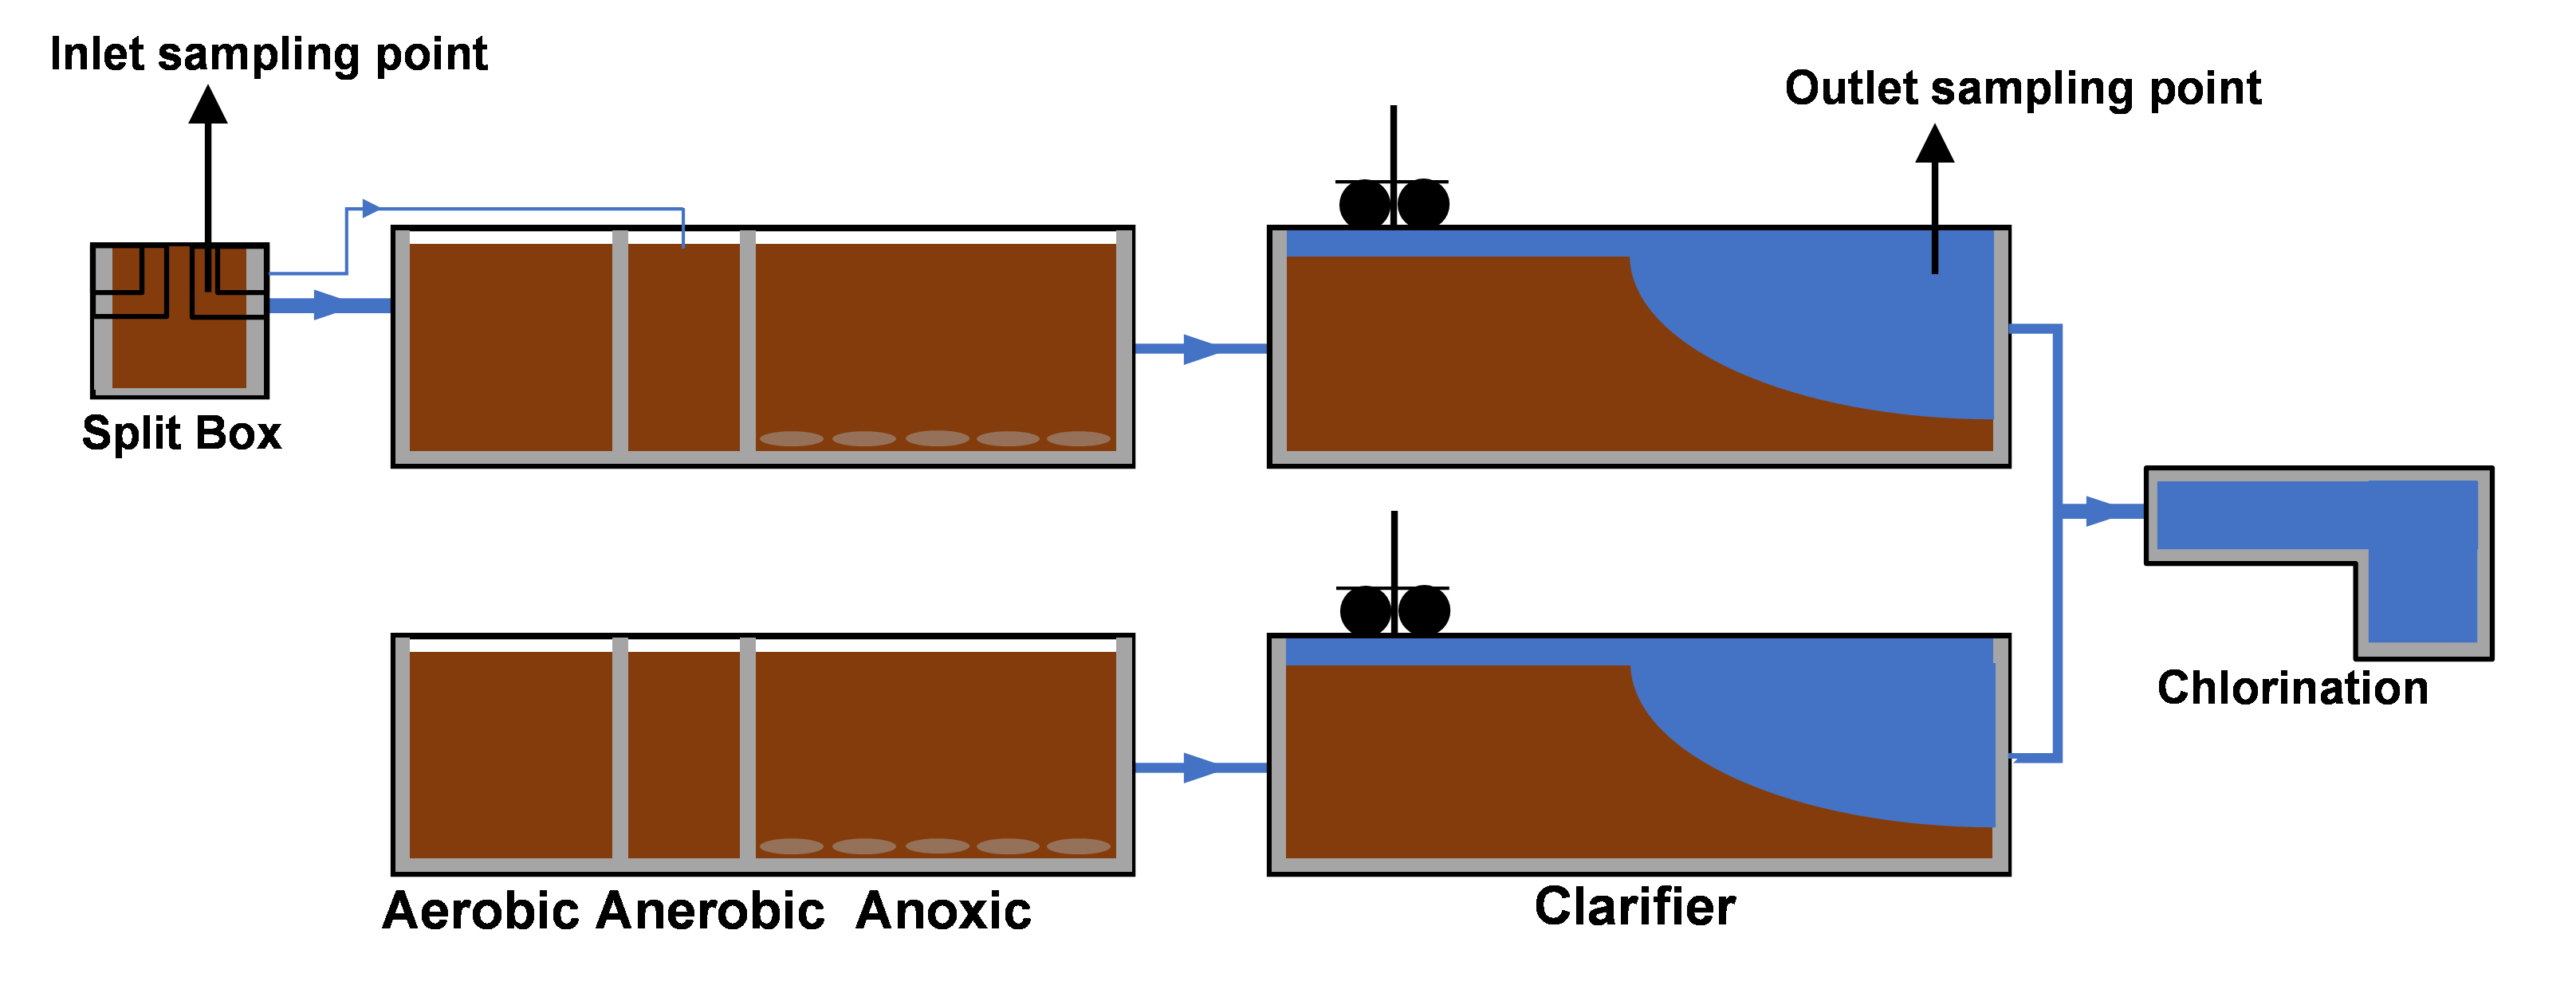
\includegraphics[width=1\linewidth]{material_and_methodology/sample_point_inlet_outlet.png}


\caption{wastewater sampling points }
\label{fig:sample_points_inlet_outlet}
\end{figure}



\subsubsection{Sludge Sampling Points}
The samples were collected from three locations, and the analyzed parameters and Number of samples from December to February are shown below:

\begin{table}[H]
\caption{Sample Details related to the sludge}
\centering
\begin{tabular}{|l|l|l|c|p{4 cm}|}
\hline
No & Sample Location & Sample Description & No of samples & Tested Parameters \\
\hline
01 & Sludge storage tank & Thickened sludge & 1 & TSS \\
\hline
02 & Dewatered Unit & Reject water & 1 & TSS \\
\hline
03 & Dewatered Unit & Dewatered sludge & 3 & Moisture content \\
\hline
04 & Sludge drying bed & Dried sludge & 15 & Moisture content , Volatile matter content \\
\hline
\end{tabular}

\label{table:sample_details}
\end{table}

\begin{figure}[H]
\centering
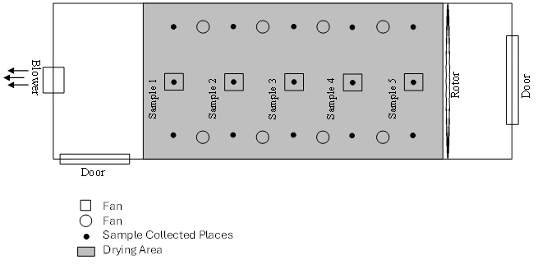
\includegraphics[width=1\linewidth]{material_and_methodology/samples_collected_points_in_the_drying_bed.png}
\caption{Samples collected points in the drying bed.}
\label{fig:samples_collected_points}
\end{figure}


\subsubsection{Determination of Total Suspended Solid}
Two dry and clean glass microfiber filter papers with watch glasses were weighed and samples 01 and 02 were filtered using pre-weighed glass microfiber filter papers. Each filtered paper was kept on the watch glass and stored at 105 ℃ for 1 hour. After 1 hour, samples were removed and placed in a desiccator until getting constant weight. Then, samples were weighted and \ac{TSS} was calculated using the below formula:

\begin{equation}
    \text{TSS} = \dfrac{\text{Weight of suspended solid (\unit{mg})}}{\text{Volume of water filtered (\unit{l})}}
\end{equation}

\subsubsection{Determination of Moisture Content}
Dry and clean aluminum foil containers were weighted and used to tare the balance. Samples 03 and 04 were added to each container and measured the weight. Then the samples were stored at 105 °C for 18 hours. After 18 hours, samples were removed and placed in a desiccator until getting constant weight. Then, Samples were weighted and moisture content was calculated using the below formula:

\begin{equation}
    \text{Moisture Content} = \dfrac{\text{Wet weight of sludge (\unit{g})} - \text{Dry weight of sludge (\unit{g})}}{\text{Wet weight of sludge (\unit{g})}} \times 100\%
\end{equation}

\subsubsection{Determination of Sludge Volatile  Matter Content}
A dry and clean porcelain disk was weighted and tared the balance. Sample 04 was added to the disk, and the weight was measured. The sample was stored at 105 °C for 18 hours. The sample was placed in a desiccator until getting constant weight and weighted. Then, sample was stored at 550 °C for 40 minutes and restored in as desiccator until getting constant weight and reweighted. \ac{SVMC} was calculated using below formula:

\begin{equation}
    \text{\ac{SVMC}} = \dfrac{\text{Weight at 105} ^\circ C \left( \unit{g} \right) - \text{Weight at 550} ^\circ C\left( \unit{g} \right) } {\text{Weight at 105} ^\circ C  \left( \unit{g} \right)}\times 100\%
\end{equation}

\subsubsection{Determination of Removal Efficiency}
The current efficiency of the plant was estimated using below formula:

\begin{equation}
    \text{Removal Efficiency} = \dfrac{\text{influent} \left( \unit{mg/l} \right) - \text{effluent} \left( \unit{mg/l} \right) }{\text{influent} \left( \unit{mg/l} \right)}
\end{equation}
\\

By regression analysis, the Correlation between the \ac{BOD5} and the \ac{TSS} was established \cite{Kumar2010}.

 